% tikz_colordiffs.tex

\begin{tikzpicture}

\begin{groupplot}[
		group style = {
			group name = dE,
			group size = 3 by 1,
			vertical sep = .25cm,
			horizontal sep = .25cm, 
			},
		width = 4.5cm,
		height = 4cm,
		enlargelimits = 0.05,
		simpleax1,
		ytick = {0,50,100},
		xticklabel = \empty,
		xmin = 0.5,
		xmax = 10.5,
		ymin = 0,
		ymax = 100,
		scale only axis,
		enlargelimits = false,
		xtick = {1.5,...,10.5},
		xmajorgrids = true, 
		ylabel = {lightness $L$},
		xlabel style = {yshift = -0.4cm},
		]

		\nextgroupplot[xlabel = {RGB}]
		\addplot+[hcqblue, ultra thick, mark = triangle*, mark options = {thin, fill = hcqblue, draw = black}]table[y index = 1]{coldiffLight.txt};
		%\coordinate (p1) at (rel axis cs:0,0);
		

		\nextgroupplot[xlabel = {HSV}, ylabel = \empty, yticklabel = \empty]
		\addplot+[hcqblue, ultra thick, mark = triangle*,mark options = {thin, fill = hcqblue, draw = black}]table[y index = 2]{coldiffLight.txt};

		\nextgroupplot[xlabel = {Lab}, ylabel = \empty, yticklabel = \empty]
		\addplot+[hcqblue, ultra thick, mark = triangle*,mark options = {thin, fill = hcqblue, draw = black}]table[y index = 3]{coldiffLight.txt};

\end{groupplot}

\node[draw = black, thick, inner sep = 0pt, anchor = north] at (dE c1r1.south){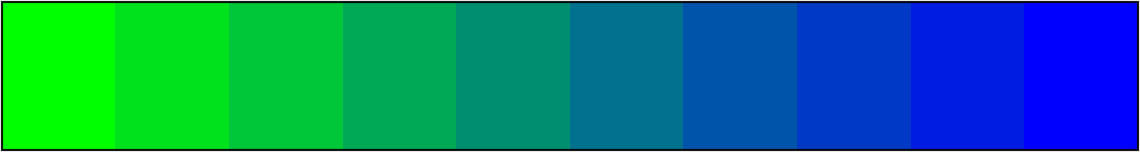
\includegraphics[width = 4.5cm]{\here/colorbarRGB.png}};
\node[draw = black, thick, inner sep = 0pt, anchor = north] at (dE c2r1.south){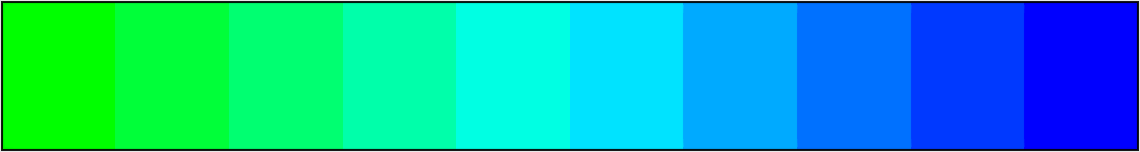
\includegraphics[width = 4.5cm]{\here/colorbarHSV.png}};
\node[draw = black, thick, inner sep = 0pt, anchor = north] at (dE c3r1.south){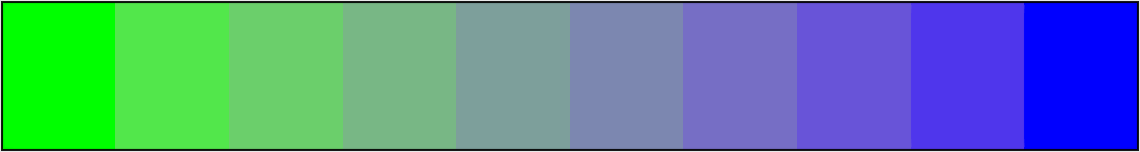
\includegraphics[width = 4.5cm]{\here/colorbarLab.png}};



\begin{groupplot}[
		group style = {
			group size = 3 by 1,
			vertical sep = .25cm,
			horizontal sep = .25cm, 
			},
		width = 4.5cm,
		height = 4cm,
		enlargelimits = 0.05,
		simpleax1,
		ytick = {0,12.5,25,37.5,50},
		xticklabel = \empty,
		yticklabels = {0,,,,50},
		xmin = 0.5,
		xmax = 10.5,
		ymin = 0,
		ymax = 50,
		ytick pos = right, 
		yticklabel pos = right,
		scale only axis,
		ylabel = {color difference},
		ylabel style = {yshift = 0.2cm},
		enlargelimits = false,
		xtick = {1.5,...,10.5},
		legend style = {
			at = {(0.5,1)},
			anchor = south,
			legend1},
		legend columns = 3
		]


		\nextgroupplot[ylabel = \empty, yticklabel = \empty]
		\addplot+[hcqyellow, ultra thick, mark options = {thin, fill = hcqyellow, draw = black}]table[y index = 1]{coldiffLab.txt};
		\addplot+[hcqred, ultra thick, mark options = {thin, fill = hcqred, draw = black}]table[y index = 1]{coldiff2000.txt};

		\addlegendentry{$\Delta E^*_{ab}$}
		\addlegendentry{$\Delta E^*_{2000}$}
		\addlegendimage{hcqblue, ultra thick, mark = triangle*, mark options = {thin, fill = hcqblue, draw = black}};
		\addlegendentry{$L$};
		

		\nextgroupplot[ylabel = \empty, yticklabel = \empty]
		\addplot+[hcqyellow, ultra thick, mark options = {thin, fill = hcqyellow, draw = black}]table[y index = 2]{coldiffLab.txt};
		\addplot+[hcqred, ultra thick, mark options = {thin, fill = hcqred, draw = black}]table[y index = 2]{coldiff2000.txt};

		\addlegendentry{$\Delta E^*_{ab}$}
		\addlegendentry{$\Delta E^*_{2000}$}
		\addlegendimage{hcqblue, ultra thick, mark = triangle*, mark options = {thin, fill = hcqblue, draw = black}};
		\addlegendentry{$L$};


		\nextgroupplot[]
		\addplot+[hcqyellow, ultra thick, mark options = {thin, fill = hcqyellow, draw = black}]table[y index = 3]{coldiffLab.txt};
		\addplot+[hcqred, ultra thick, mark options = {thin, fill = hcqred, draw = black}]table[y index = 3]{coldiff2000.txt};


		\addlegendentry{$\Delta E^*_{ab}$}
		\addlegendentry{$\Delta E^*_{2000}$}
		\addlegendimage{hcqblue, ultra thick, mark = triangle*, mark options = {thin, fill = hcqblue, draw = black}};
		\addlegendentry{$L$};

	\end{groupplot}

	\node[text width=1em, anchor=west]at(dE c1r1.north west){\subcaptionbox{\label{dEa}}{}};
	\node[text width=1em, anchor=west]at(dE c2r1.north west){\subcaptionbox{\label{dEb}}{}};
	\node[text width=1em, anchor=west]at(dE c3r1.north west){\subcaptionbox{\label{dEc}}{}};
\end{tikzpicture}
